

With a project as complex as ours, we needed to propose a schedule for each team member to turn their parts in, a system for sharing files and method of team communication.

\begin{itemize}
\item Timeline - Gantt Chart using Excel
More about the Gantt Chart is explained in the section \ref{sec:timeline}

\item Data management - Google Drive and Github
Although Github was more suited to collaborative work, we opted to use Google Drive in order to use a platform accessiblile to all team members. However, Google Drive proved to be a problem as it synced temporary files as well as permanent files, which caused issues with references inside an assembly. 
We would not reccommend using Google Drive in the future for said reason. At the end of the project, we used Github to sync Solidworks files together and to create our report.
We have two repositories for the project and the report.
\begin{itemize}
\item ME1770 files  - \url{https://github.com/vishakhkumar/ME1770}
\item ME1770 report - \url{https://github.com/vishakhkumar/ME1770Report}
\end{itemize}

\end{itemize}

\subsection{Part Distribution}
\subsubsection{Allocating subsystems among team members}

An important element of team success lies in allocating tasks to team members equitably. We kept in mind two factors while allocating tasks:

  - the set of tasks that has to be completed (which may be one task or it may be several) and
  - the set of individuals (the team members) able to complete them.

Given each team member's skill level and complexity of the part, we assigned tasks as shown in the Project Proposal (I forgot the table number).

Further description

Since the cockpit and the controls were interrelated task, it was decided to allocate both tasks to the same person.

This probably should be filled out more.


\subsection{Timeline} \label{sec:timeline}
 Planning our project was simple using Gantt chart created in an Excel sheet. We opted to finish our tasks earlier than suggested by the Gantt chart provided to us by our instructor due to our experience with Solidworks and inreased workload at the end of the semester from other subjects. 
We've included an image of our Gantt chart in the figure \ref{fig:GanttChart} on page \pageref{fig:GanttChart}.\\
 A detailed view of our timeline can be found at \url{https://github.com/vishakhkumar/ME1770}

\begin{figure}[!ht]
\centering
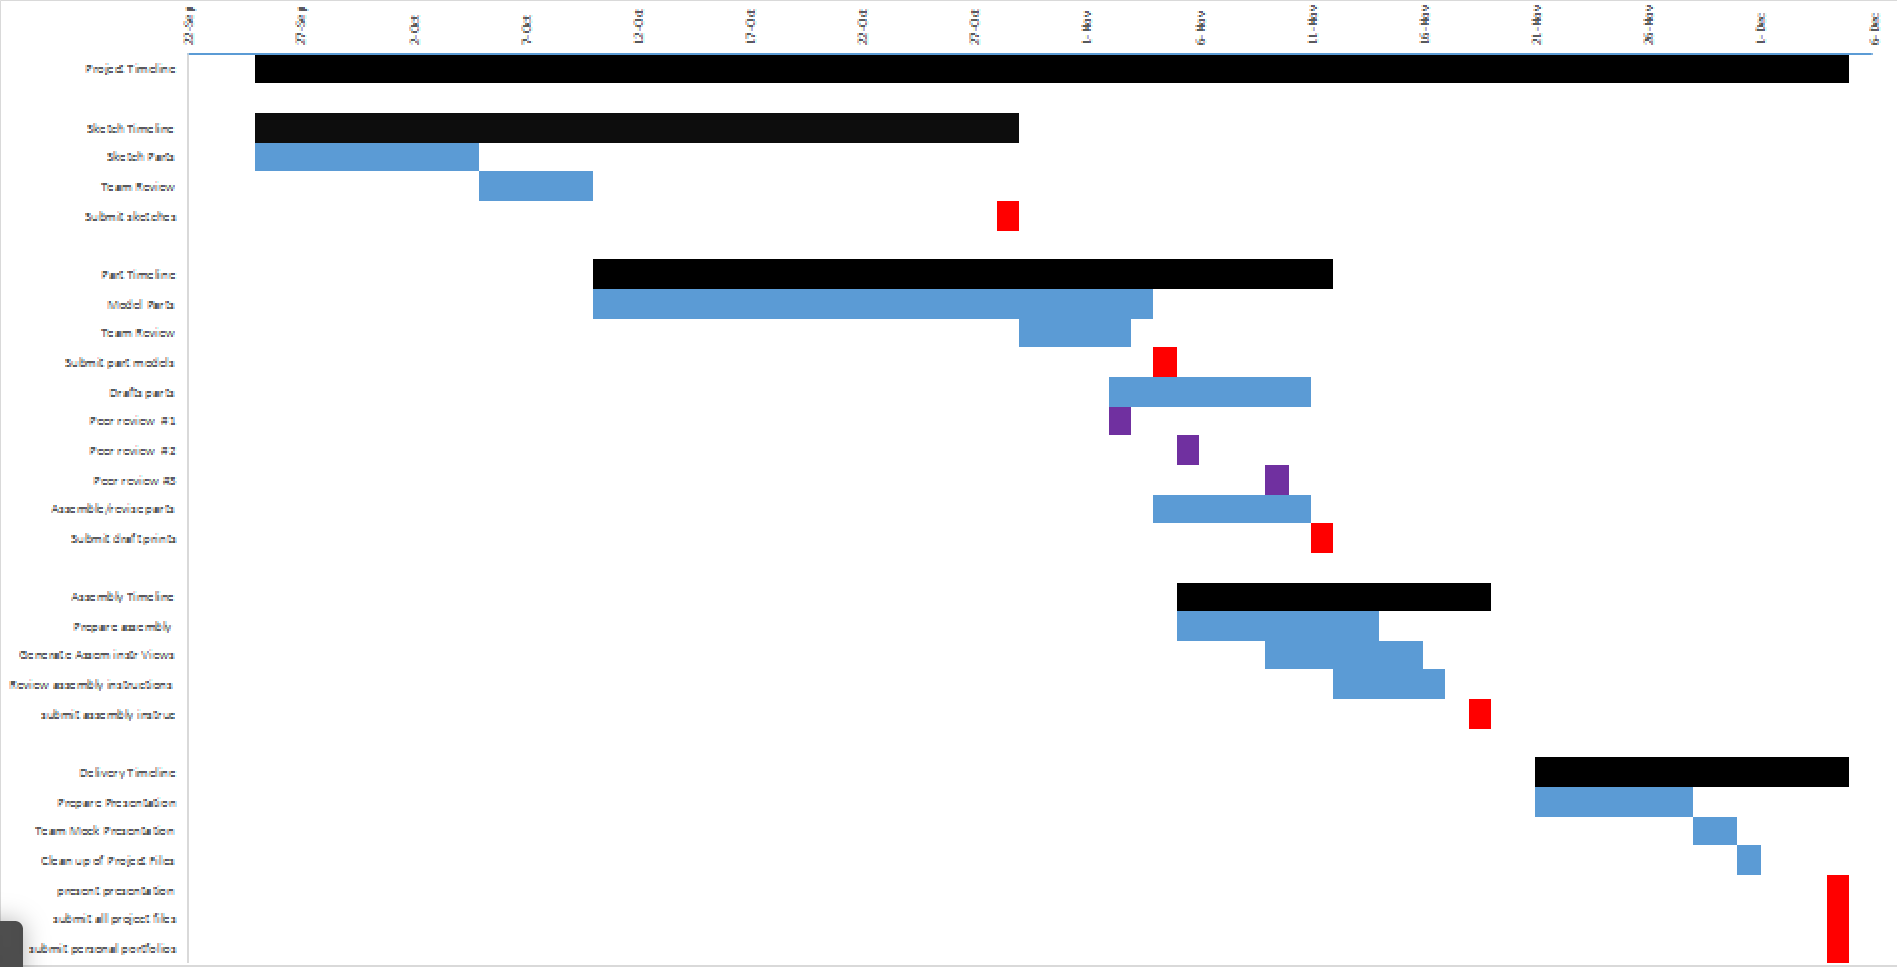
\includegraphics[angle=90,height=\textheight]{a-1-1-ProjectIdeation/b-2-ProjectManagement/Timeline.png}
\caption{Gantt Chart}
\label{fig:GanttChart}
\end{figure}

\clearpage
